\documentclass[aspectratio=169]{beamer}
%[handout]

\usetheme[progressbar=frametitle]{metropolis}
\usepackage{appendixnumberbeamer}

\usepackage[utf8]{inputenc}
\usepackage[T1]{fontenc}

\usepackage[brazil]{babel}
\usepackage[outputdir=..]{minted}
\usepackage{xcolor}
\usepackage{soul} % strikethrough
\usepackage{advdate}
\usepackage{graphicx}
\graphicspath{{figs/}}
\usepackage{graphbox}

\usepackage[ampersand]{easylist}

\usepackage{multirow}
\usepackage{multicol}
\usepackage{subcaption}

\usepackage{pgf,tikz}
\usetikzlibrary{shapes,arrows,positioning}
\usetikzlibrary{circuits.logic.US}
\usetikzlibrary{matrix,calc}

\usepackage{karnaugh-map}

\usepackage{pgfpages}
\setbeameroption{hide notes} % Only slides
% \setbeameroption{show only notes} % Only notes
% \setbeameroption{show notes on second screen=right} % Both

% \graphicspath{{../figs/}}

\definecolor{bgc}{rgb}{0.95,0.9,0.95}
\definecolor{links}{HTML}{2A7F7F}
\hypersetup{colorlinks,linkcolor=,urlcolor=links}

\newminted{verilog}{fontsize=\scriptsize, 
    linenos,
    numbersep=8pt,
    bgcolor=bgc,
    tabsize=4,
    framesep=3mm} 
    %frame=lines,

\newcommand{\verilog}[1]{\verilogf{#1}{\footnotesize}}

\newcommand{\verilogf}[2]{\inputminted[fontsize=#2, 
    linenos,
    tabsize=2,
    numbersep=4pt,
    bgcolor=bgc,
    framesep=3mm]{verilog}{../codes/#1.v}
}

\newminted{nasm}{fontsize=\scriptsize, 
		   linenos,
		   numbersep=8pt,
           bgcolor=bgc,
		   framesep=3mm} 

\usepackage{booktabs}
\usepackage[scale=2]{ccicons}

\usepackage{pgfplots}
\usepgfplotslibrary{dateplot}

\usepackage{hyperref}


\usepackage{xspace}
\newcommand{\themename}{\textbf{\textsc{metropolis}}\xspace}



\usepackage{pifont}% http://ctan.org/pkg/pifont
\newcommand{\cmark}{\ding{51}}%
\newcommand{\xmark}{\ding{55}}%

% \tiny	
% \scriptsize
% \footnotesize
% \small	
% \normalsize	
% \large	
% \Large	
% \LARGE	
% \huge	
% \Huge	



\newminted{python}{fontsize=\scriptsize, 
		   linenos,
		   breaklines,
		   numbersep=8pt,
           tabsize=2,
		   framesep=3mm} 
		   
\newminted{verilog}{fontsize=\scriptsize, 
		   linenos,
		   breaklines,
		   numbersep=8pt,
           tabsize=2,
		   framesep=3mm} 
		   




\definecolor{bgc}{rgb}{0.95,0.9,0.95}
\definecolor{links}{HTML}{2A7F7F}
\hypersetup{colorlinks,linkcolor=,urlcolor=links}


% \usepackage[style=apa]{biblatex}
% \addbibresource{mm.bib}


% \author{\large Prof. Ricardo Menotti (\href{mailto:menotti@ufscar.br}{menotti@ufscar.br})}

\newcommand{\newauthor}[2]{
  \parbox{0.50\textwidth}{
    \texorpdfstring
      {
        \centering
        \small #1 \newline
        {\scriptsize{\urlstyle{same}\href{mailto:#2}{#2}\urlstyle{tt}}}
      }
      {#1} \newline
  }
}

\author{
  \newauthor{Prof. Ricardo Menotti}{menotti@ufscar.br}
\and \newauthor{Prof. Luciano de Oliveira Neris}{lneris@ufscar.br}  
%\and \newauthor{Prof. Artino Quintino da Silva Filho}{artino@ufscar.br}
% \and \newauthor{Prof. Maurício Figueiredo}{mauricio@ufscar.br}
% \and \newauthor{Prof. Edilson Kato}{kato@ufscar.br}
% \and \newauthor{Prof. Roberto Inoue}{rsinoue@ufscar.br}
}

\date{Atualizado em: \today}

\institute{\large \textbf{Departamento de Computação} \\
Centro de Ciências Exatas e de Tecnologia \\
Universidade Federal de São Carlos}

\title{Lógica Digital (1001351)}

\titlegraphic{\hfill
\includegraphics[height=1.5cm]{LogoUfscar}}



\setbeameroption{hide notes} % Only slides
%\setbeameroption{show only notes} % Only notes
% \setbeameroption{show notes on second screen=right} % Both
% See: https://gist.github.com/andrejbauer/ac361549ac2186be0cdb

\subtitle{Funções e Circuitos Lógicos} % 

\begin{document}

\begin{frame}
	\titlepage
\end{frame} 

% Uncomment if you want a summary slide
% \begin{frame}{Conteúdo}
% 	\tableofcontents
% \end{frame}


\section{Variáveis e Funções}

\frame{     \centering
    \frametitle{Uma variável binária}
    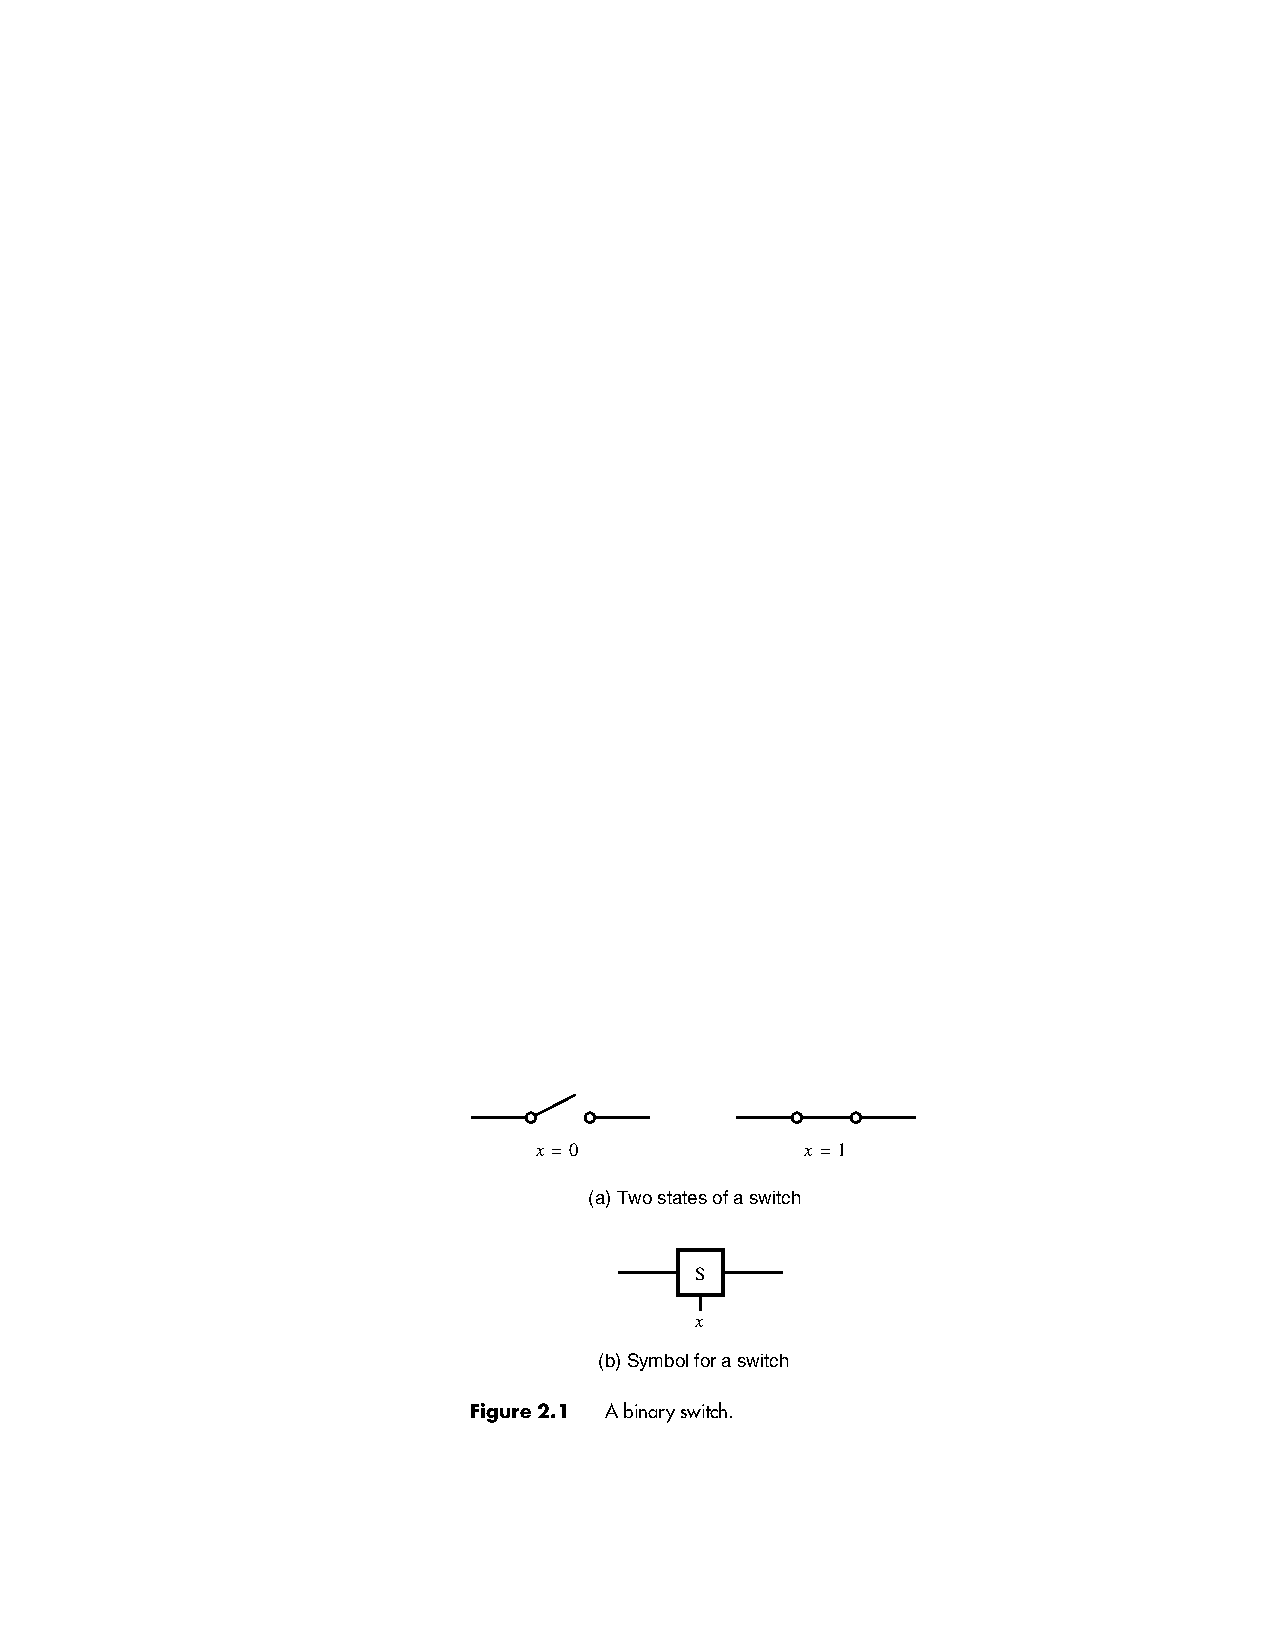
\includegraphics{VerilogFig2_1}
}

\frame{     \centering
    \frametitle{Uma variável binária}
    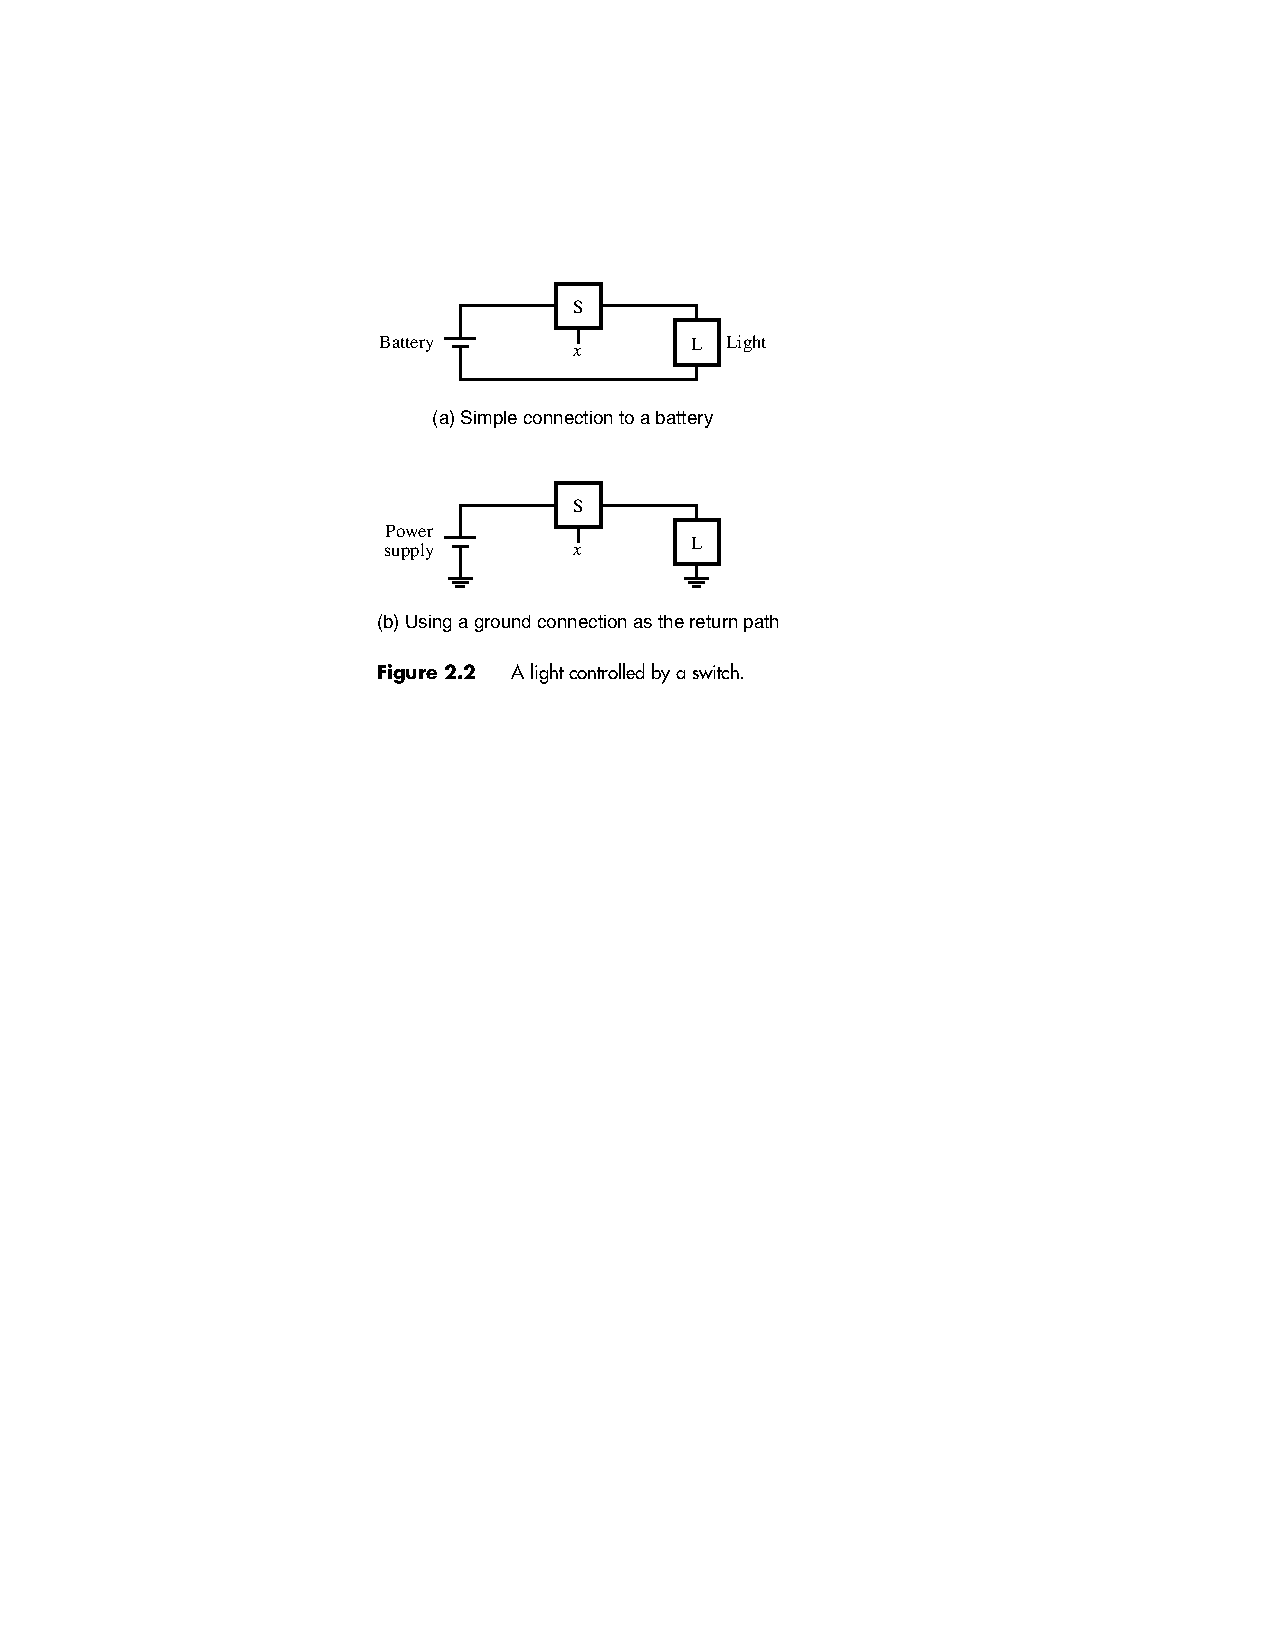
\includegraphics{VerilogFig2_2}
}

\begin{frame}{Funções lógicas E (série) e OU (paralelo)} 
    \begin{columns}
        \begin{column}{0.60\textwidth}
            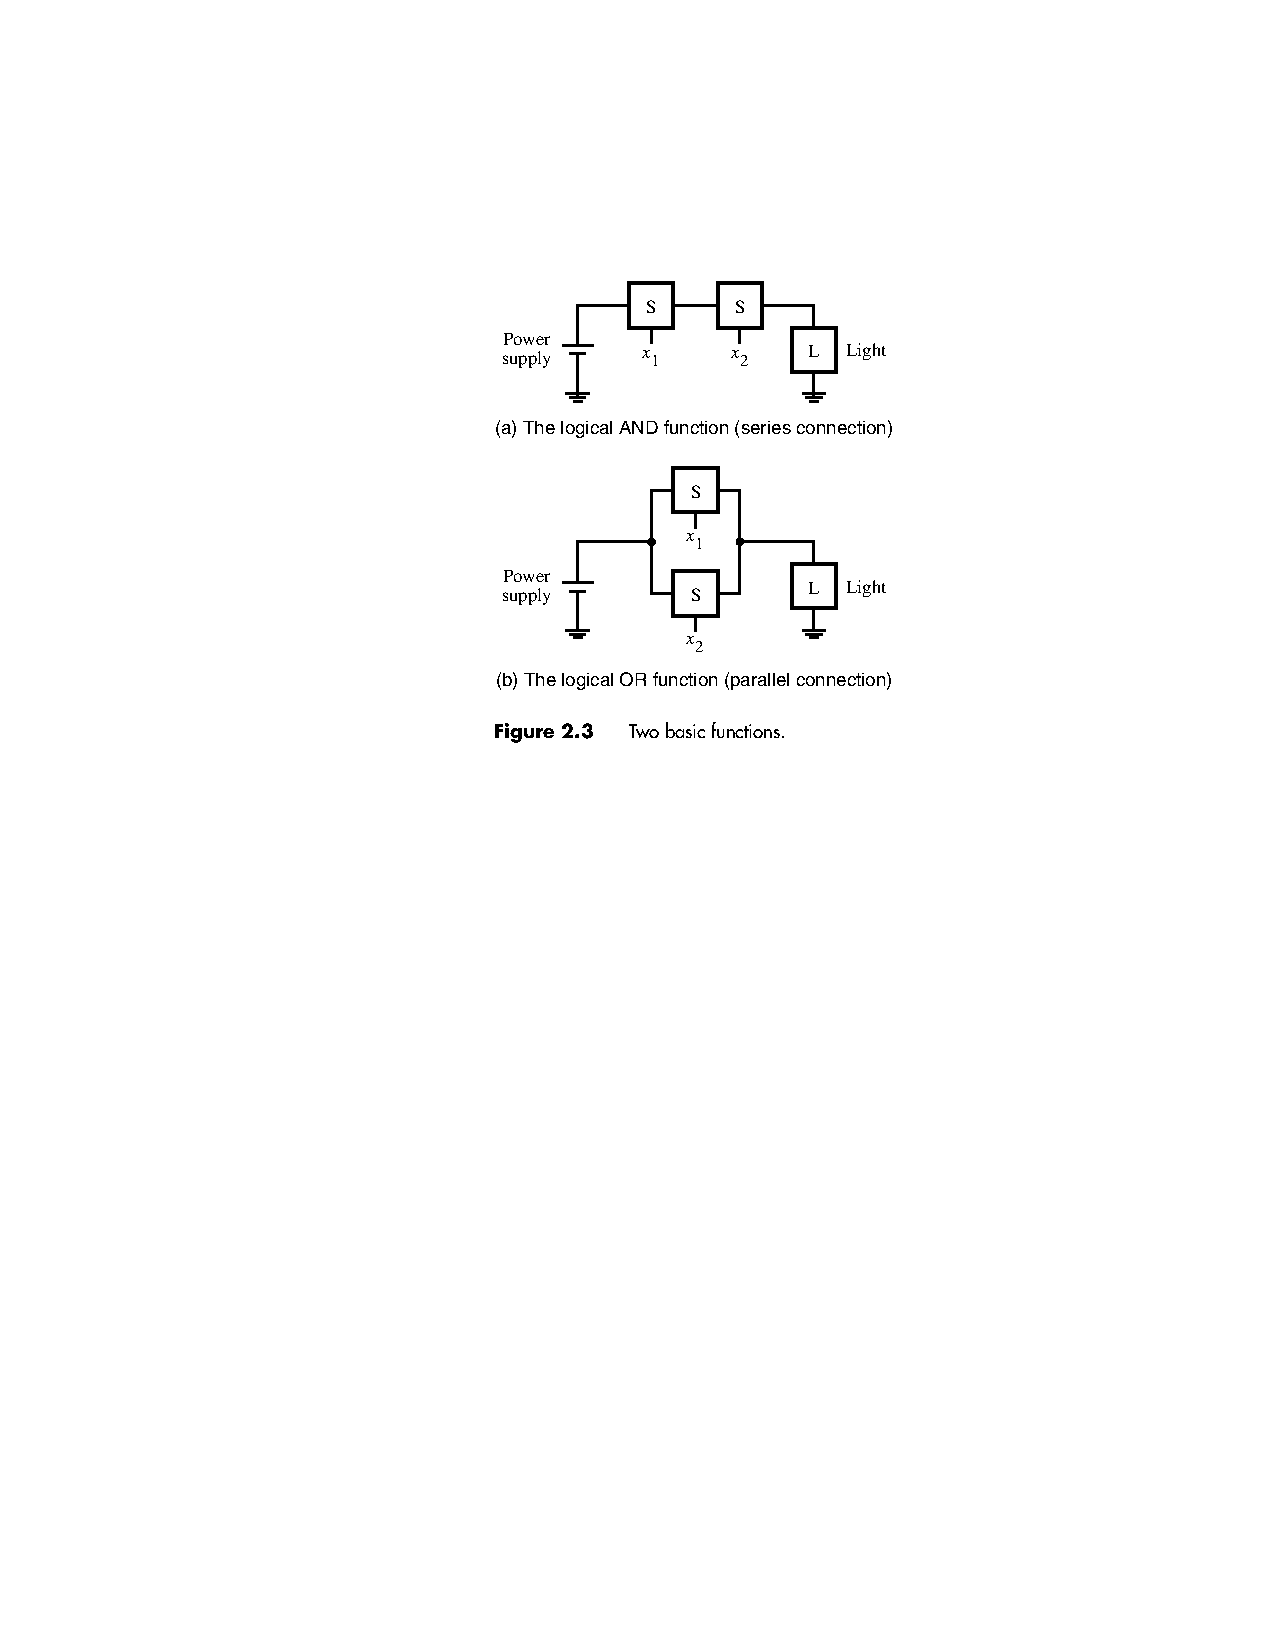
\includegraphics[width=\textwidth]{VerilogFig2_3}
        \end{column}        
        \begin{column}{0.40\textwidth}
            $L(x_1,x_2) = x_1.x_2$ \\
            \textit{onde} \\
            $L = 1$ se $x_1 = 1$ \textbf{E} $x_2 = 1$, \\
            $L = 0$ \textit{caso contrário.} \\
            \vspace{1cm}
            $L(x_1,x_2) = x_1 + x_2$ \\
            \textit{onde} \\
            $L = 1$ se $x_1 = 1$ \textbf{OU} $x_2 = 1$ \textbf{OU} $x_1 = x_2 = 1$, \\
            $L = 0$ se $x_1 = x_2 = 0$. \\
            \vspace{1cm}
        \end{column}
    \end{columns}
\end{frame}

\begin{frame}{Combinando as funções} 
    \centering
    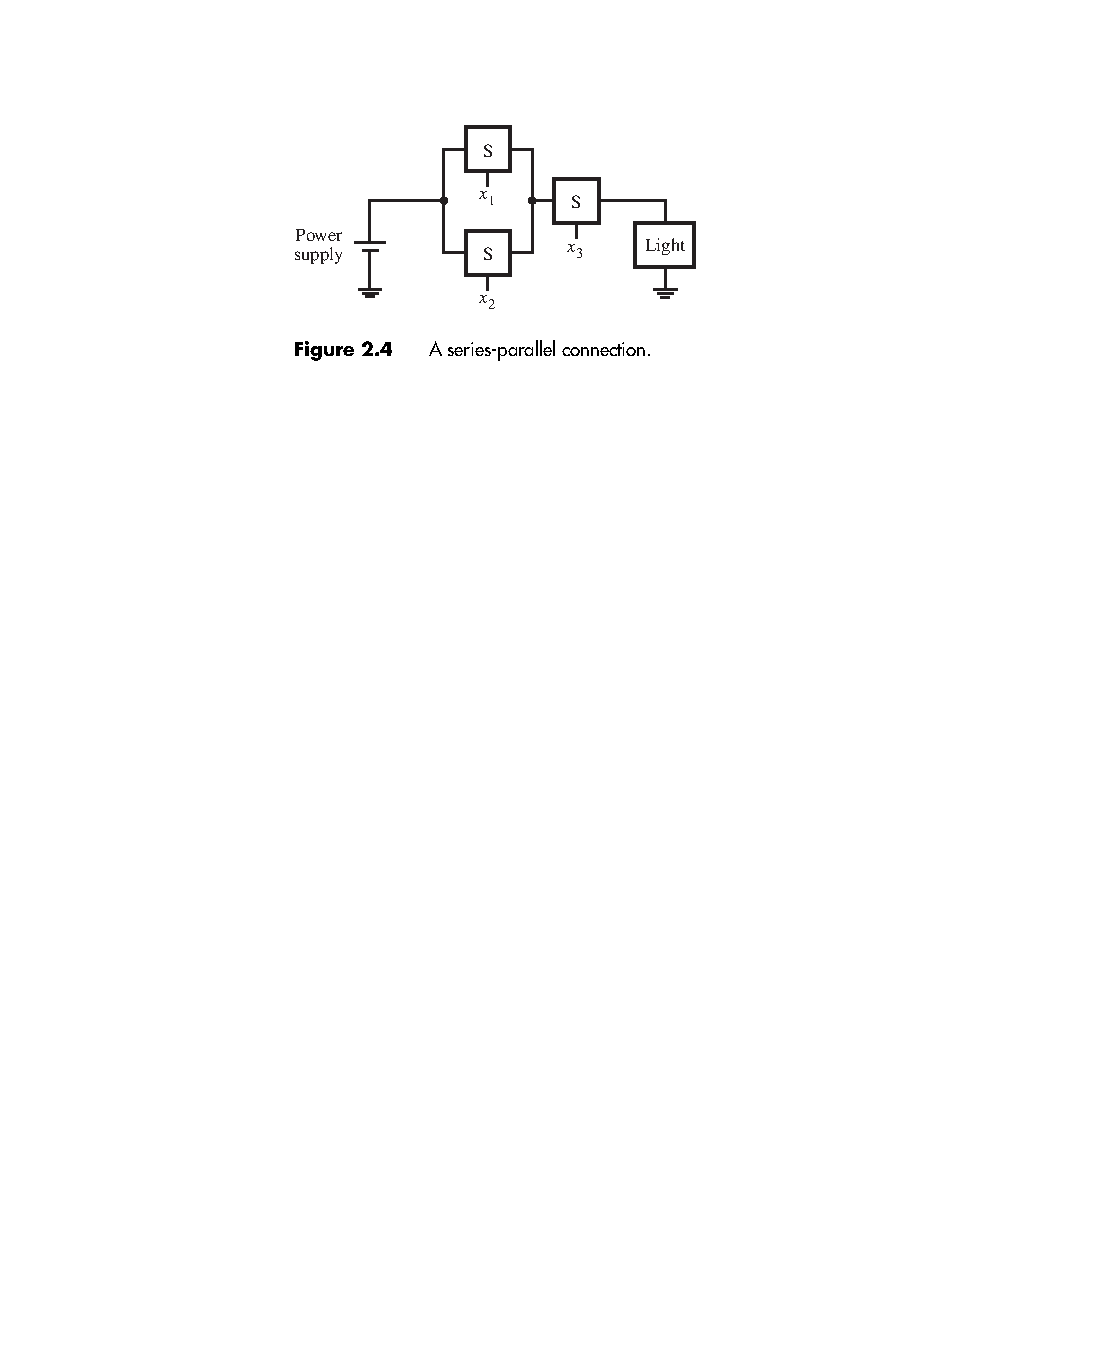
\includegraphics[width=.7\textwidth]{VerilogFig2_4} \\
    $L(x_1,x_2,x_3) = (x_1 + x_2).x_3$ 
\end{frame}

\frame{     \centering
    \frametitle{Função lógica NÃO (inversão ou complemento)}
    \begin{columns}
        \begin{column}{0.60\textwidth}
            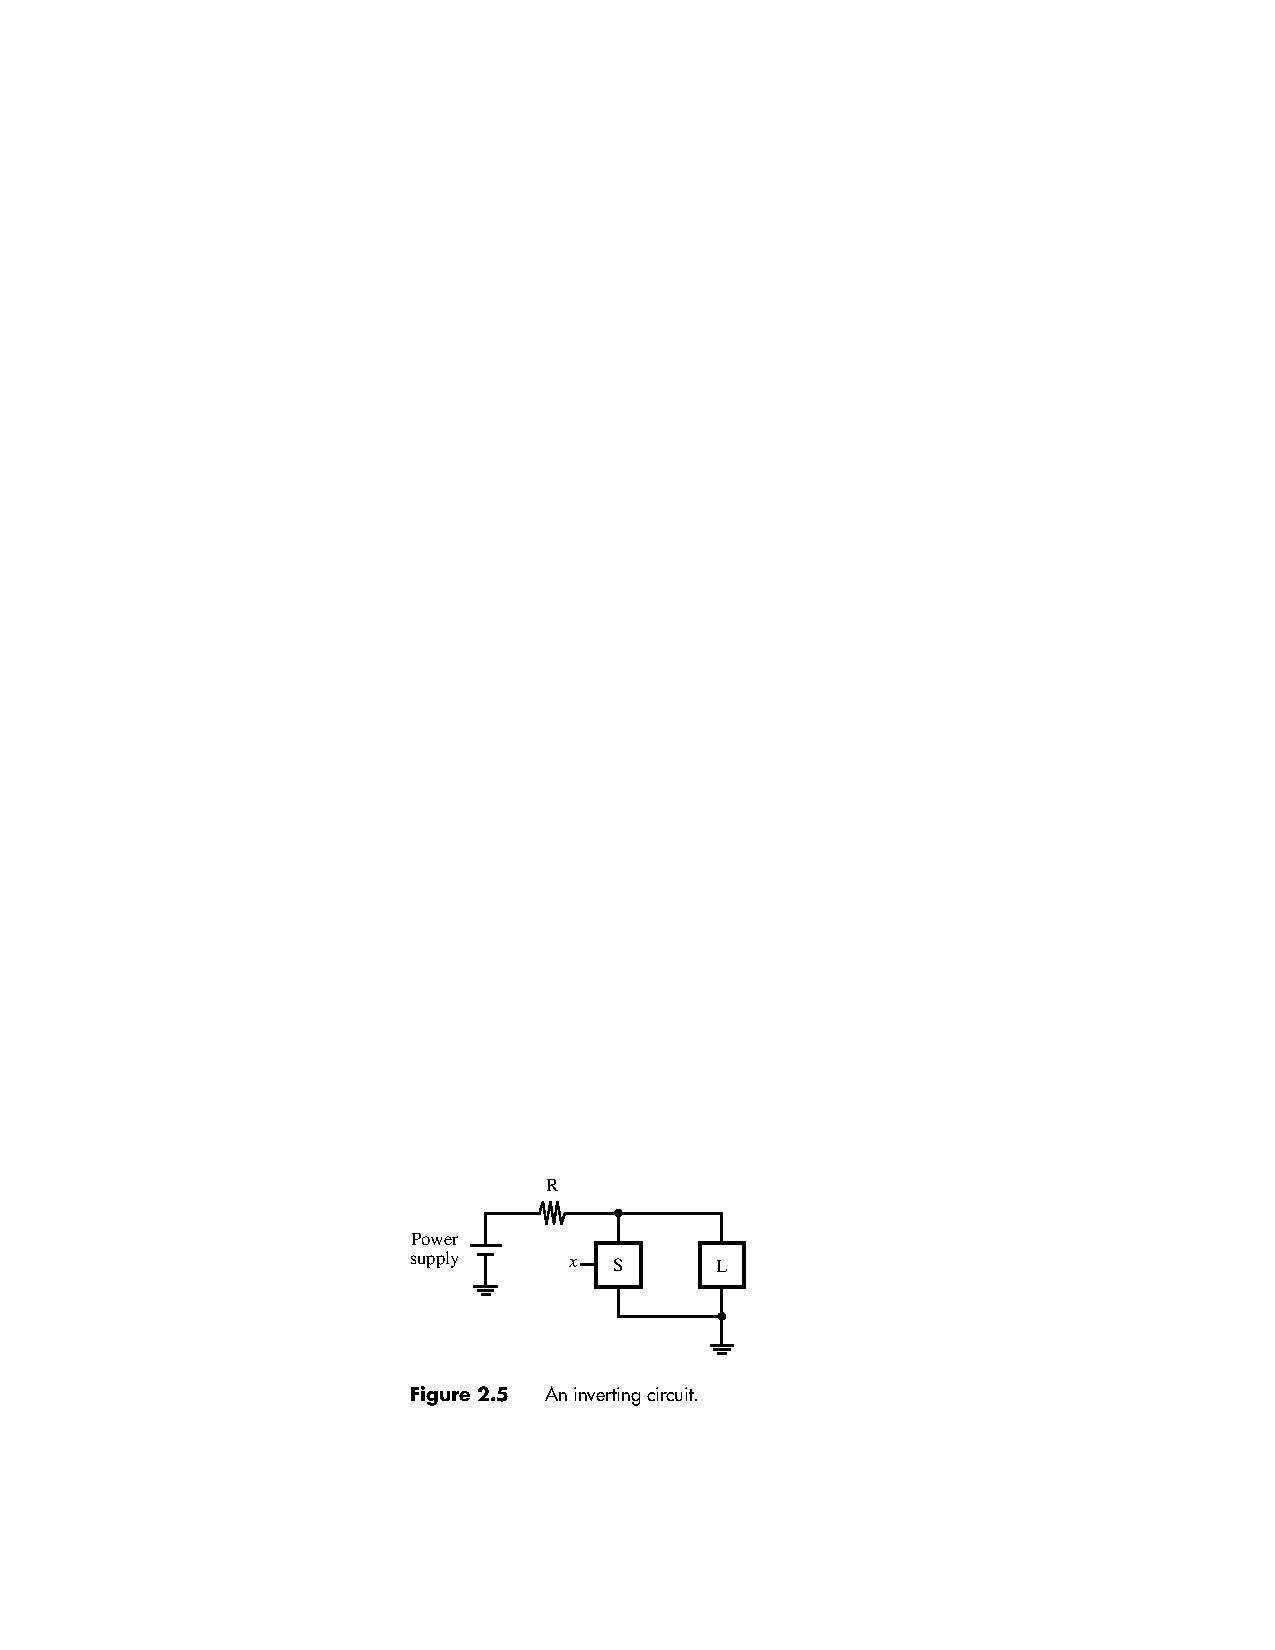
\includegraphics[width=\textwidth]{VerilogFig2_5}
        \end{column}        
        \begin{column}{0.40\textwidth}
            $L(x) = \overline{x}$ \\
            \textit{onde} \\
            $L = 1$ se $x = 0$, \\
            $L = 0$ se $x = 1$. \\
        \end{column}
    \end{columns}
    representações possíveis: $\overline{x}=x'=~!x=~\sim{x}= $ NOT$x$ \\
    para $f(x_1,x_2)=x_1+x_2$, temos seu complemento $\overline{f}(x_1,x_2)=\overline{x_1+x_2}$\\
    $=(x_1+x_2)'=~!(x_1+x_2)=~\sim{(x_1+x_2)}= $ NOT$(x_1+x_2)$ \\
}


\frame{     \centering
    \frametitle{Tabela Verdade}
    \begin{table}[]
        \centering 
        \begin{tabular}{cc||c|c} % center, left or right 
            \hline
            $x_1$ & $x_2$ & $x_1.x_2$ & $x_1+x_2$\\
            \hline
            \hline
            $0$ & $0$ & $0$ & $0$ \\
            $0$ & $1$ & $0$ & $1$ \\
            $1$ & $0$ & $0$ & $1$ \\
            $1$ & $1$ & $1$ & $1$ \\
            \hline
        \end{tabular} \\
        \vspace{1cm}
        Tabela Verdade para as funções lógicas AND e OR
    \end{table}
}

\frame{     \centering
    \frametitle{Lógica Proposicional}
    \begin{table}[]
        \centering 
        \begin{tabular}{cc||c|c|c|c|c} % center, left or right 
            \hline
            \multicolumn{2}{c||}{\scriptsize \textit{proposições}} & \scriptsize \textit{negação} & \scriptsize \textit{conjunção} & \scriptsize \textit{disjunção} & \scriptsize \textit{implicação} & \scriptsize \textit{equivalência} \\
            $p$ & $q$ & $\sim{p}$ & $p \wedge q$ & $p \vee q$ & $p \rightarrow q$ & $p \Leftrightarrow q$ \\
            \hline
            \hline
            $0$ & $0$ &     & $0$ & $0$  & $1$ & $1$ \\
            $0$ & $1$ & $1$ & $0$ & $1$  & $1$ & $0$ \\
            $1$ & $0$ & $0$ & $0$ & $1$  & $0$ & $0$ \\
            $1$ & $1$ &     & $1$ & $1$  & $1$ & $1$ \\
            \hline
        \end{tabular} \\
        \vspace{1cm}
        Tabela Verdade para os conectivos lógicos
        
    % \note[item]{Note that this slide is boring.}
    % \note[item]{Observe that there are no actual bullets here.}
    % \note[item]{Future work: add another bullet.}
    \end{table}
}

\frame{     \centering
    \frametitle{Tabela Verdade}
    \begin{table}[]
        \centering  
        \begin{tabular}{ccc||c|c} % center, left or right 
            \hline
            $x_1$ & $x_2$ & $x_3$ & $x_1.x_2.x_3$ & $x_1+x_2+x_3$ \\
            \hline
            \hline
            $0$  & $0$ & $0$ & $0$ & $0$ \\
            $0$  & $0$ & $1$ & $0$ & $1$ \\
            $0$  & $1$ & $0$ & $0$ & $1$ \\
            $0$  & $1$ & $1$ & $0$ & $1$ \\
            $1$  & $0$ & $0$ & $0$ & $1$ \\
            $1$  & $0$ & $1$ & $0$ & $1$ \\
            $1$  & $1$ & $0$ & $0$ & $1$ \\
            $1$  & $1$ & $1$ & $1$ & $1$ \\
            \hline
        \end{tabular} \\
        \vspace{1cm}
        Funções lógicas AND e OR com três entradas
    \end{table}
}

\frame{     \centering
    \frametitle{Tabela Verdade}
    \begin{table}[]
        \centering 
        \begin{tabular}{cc||c|c||c|c|c} % center, left or right 
            \hline
            $x_1$ & $x_2$ & $x_1+x_2$ & $\overline{x_1+x_2}$ & $\overline{x_1}$ & $\overline{x_2}$ & $\overline{x_1}+\overline{x_2}$\\
            \hline
            \hline
            \onslide<1->{$0$ & $0$ & $0$ & $1$ &} \onslide<2-3>{$1$ & $1$ &} \onslide<3>{ $1$} \\
            \onslide<1->{$0$ & $1$ & $1$ & $0$ &} \onslide<2-3>{$1$ & $0$ &} \onslide<3>{ $1$} \\
            \onslide<1->{$1$ & $0$ & $1$ & $0$ &} \onslide<2-3>{$0$ & $1$ &} \onslide<3>{ $1$} \\
            \onslide<1->{$1$ & $1$ & $1$ & $0$ &} \onslide<2-3>{$0$ & $0$ &} \onslide<3>{ $0$} \\
            \hline
        \end{tabular} \\
        \vspace{1cm}
        Provando que $\overline{f}(x_1,x_2)=\overline{x_1+x_2}\neq\overline{x_1}+\overline{x_2}$
    \end{table}
}

\section{Portas Lógicas e Circuitos Lógicos}

\begin{frame}{\insertsection} 
	\begin{itemize}
		\item As funções lógicas AND, OR e NOT podem ser usadas para implementar funções lógicas de qualquer complexidade;
		\pause
		\item Uma função complexa pode exigir muitas dessas operações básicas para sua implementação;
		\pause
		\item Cada operação lógica pode ser implementada eletronicamente com transistores, resultando em um elemento de circuito chamado de porta lógica;
		\pause
		\item Uma porta lógica tem uma ou mais entradas e uma saída que é uma função de suas entradas;
		\pause
		\item Podemos projetar um circuito lógico desenhando um esquemático, consistindo de símbolos gráficos representando as portas lógicas.
    \end{itemize}
\end{frame}

\frame{     \centering
    \frametitle{\insertsection}
    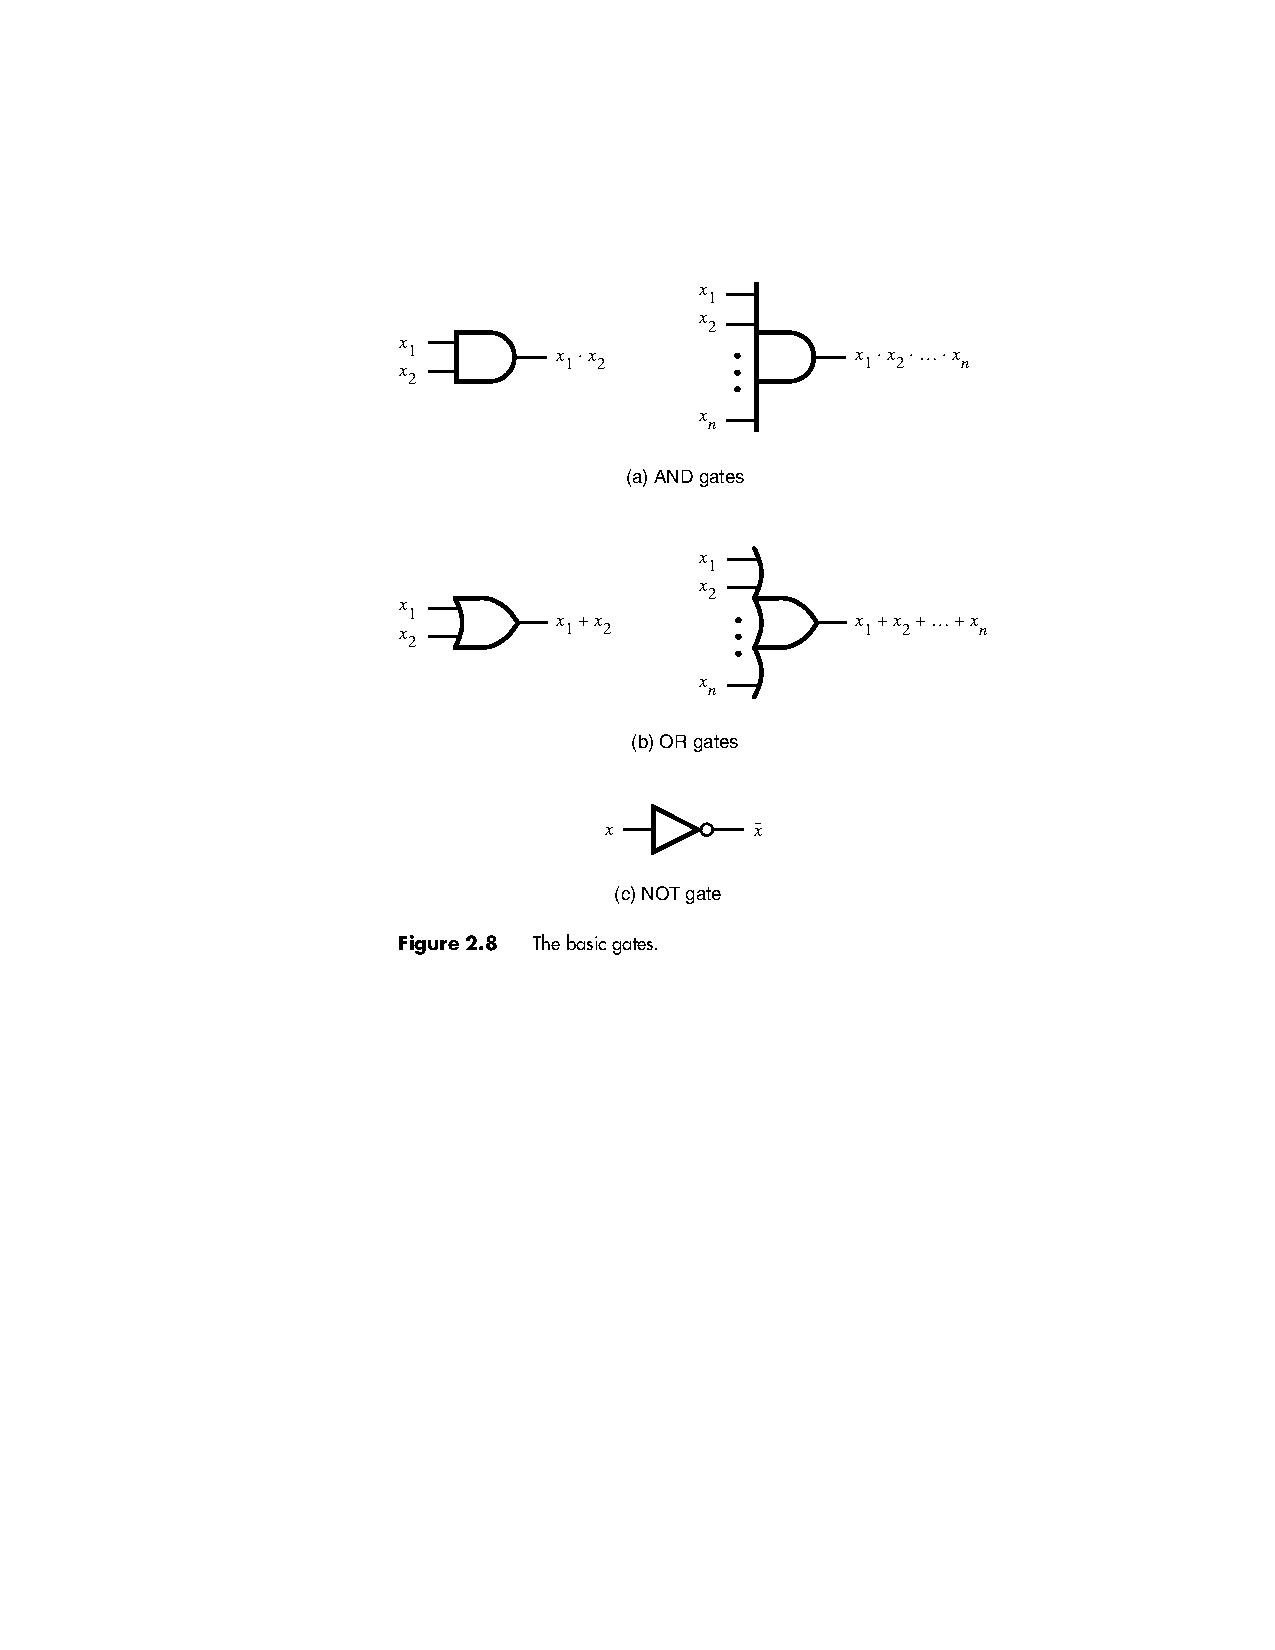
\includegraphics[scale=.7]{VerilogFig2_8}
}

\frame{     \centering
    \frametitle{\insertsection}
    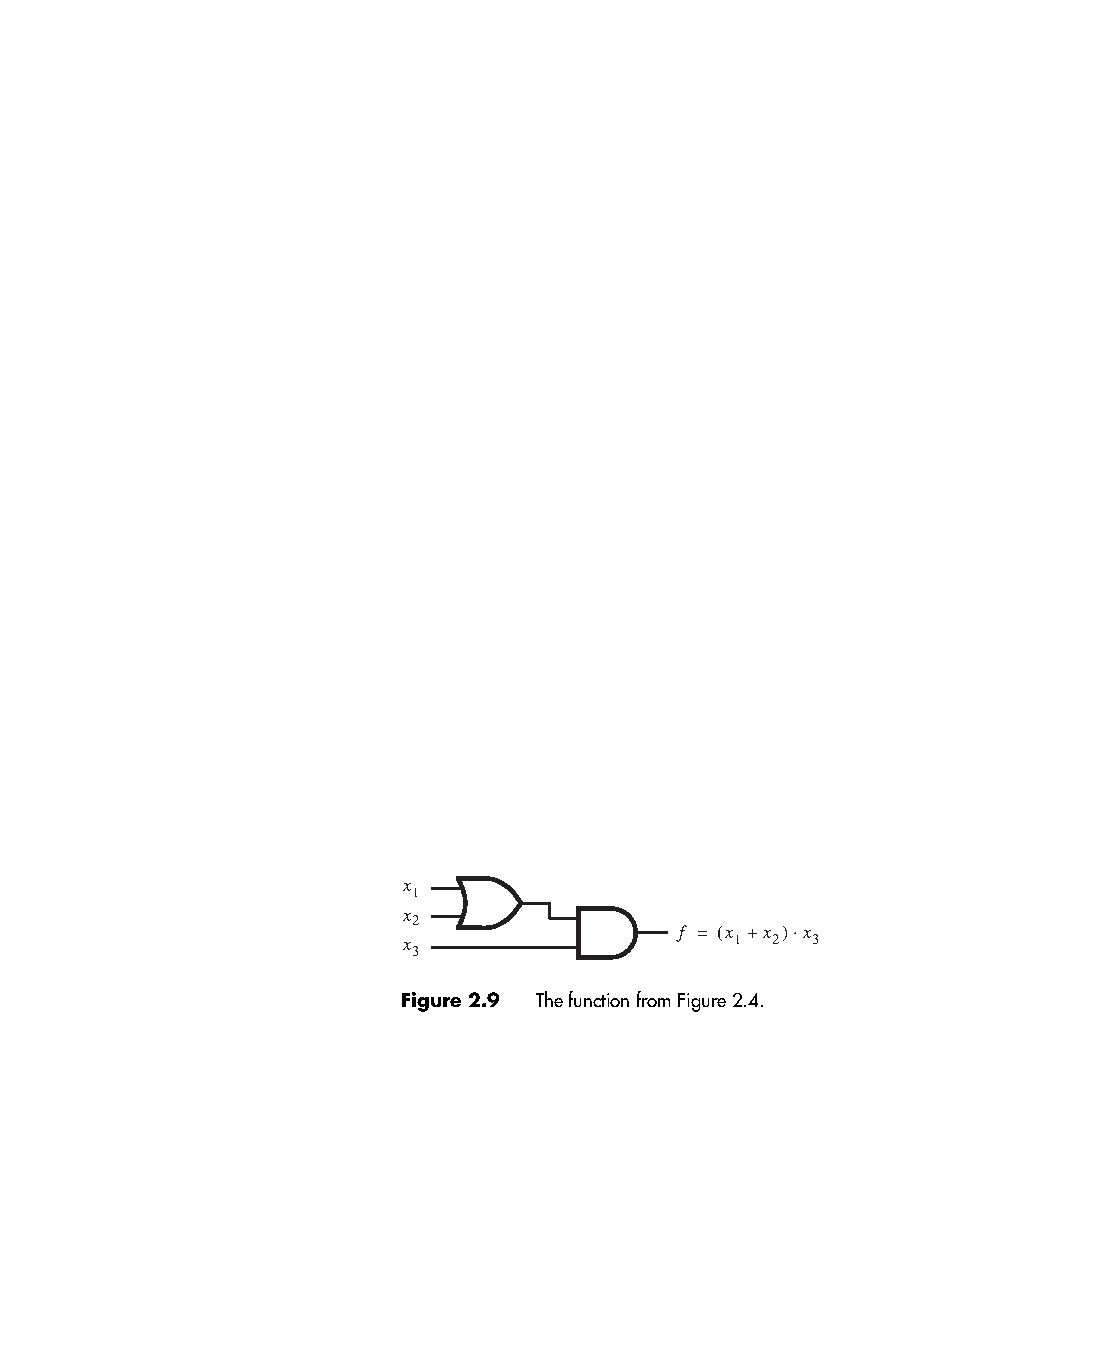
\includegraphics[width=.7\textwidth]{VerilogFig2_9}
}

\frame{     \centering
    \frametitle{Análise de um circuito lógico}
\begin{tikzpicture}
\tikzstyle{foo} = [-latex, cyan, ultra thick, rounded corners]
\node[anchor=south west,inner sep=0](image) at (0,0){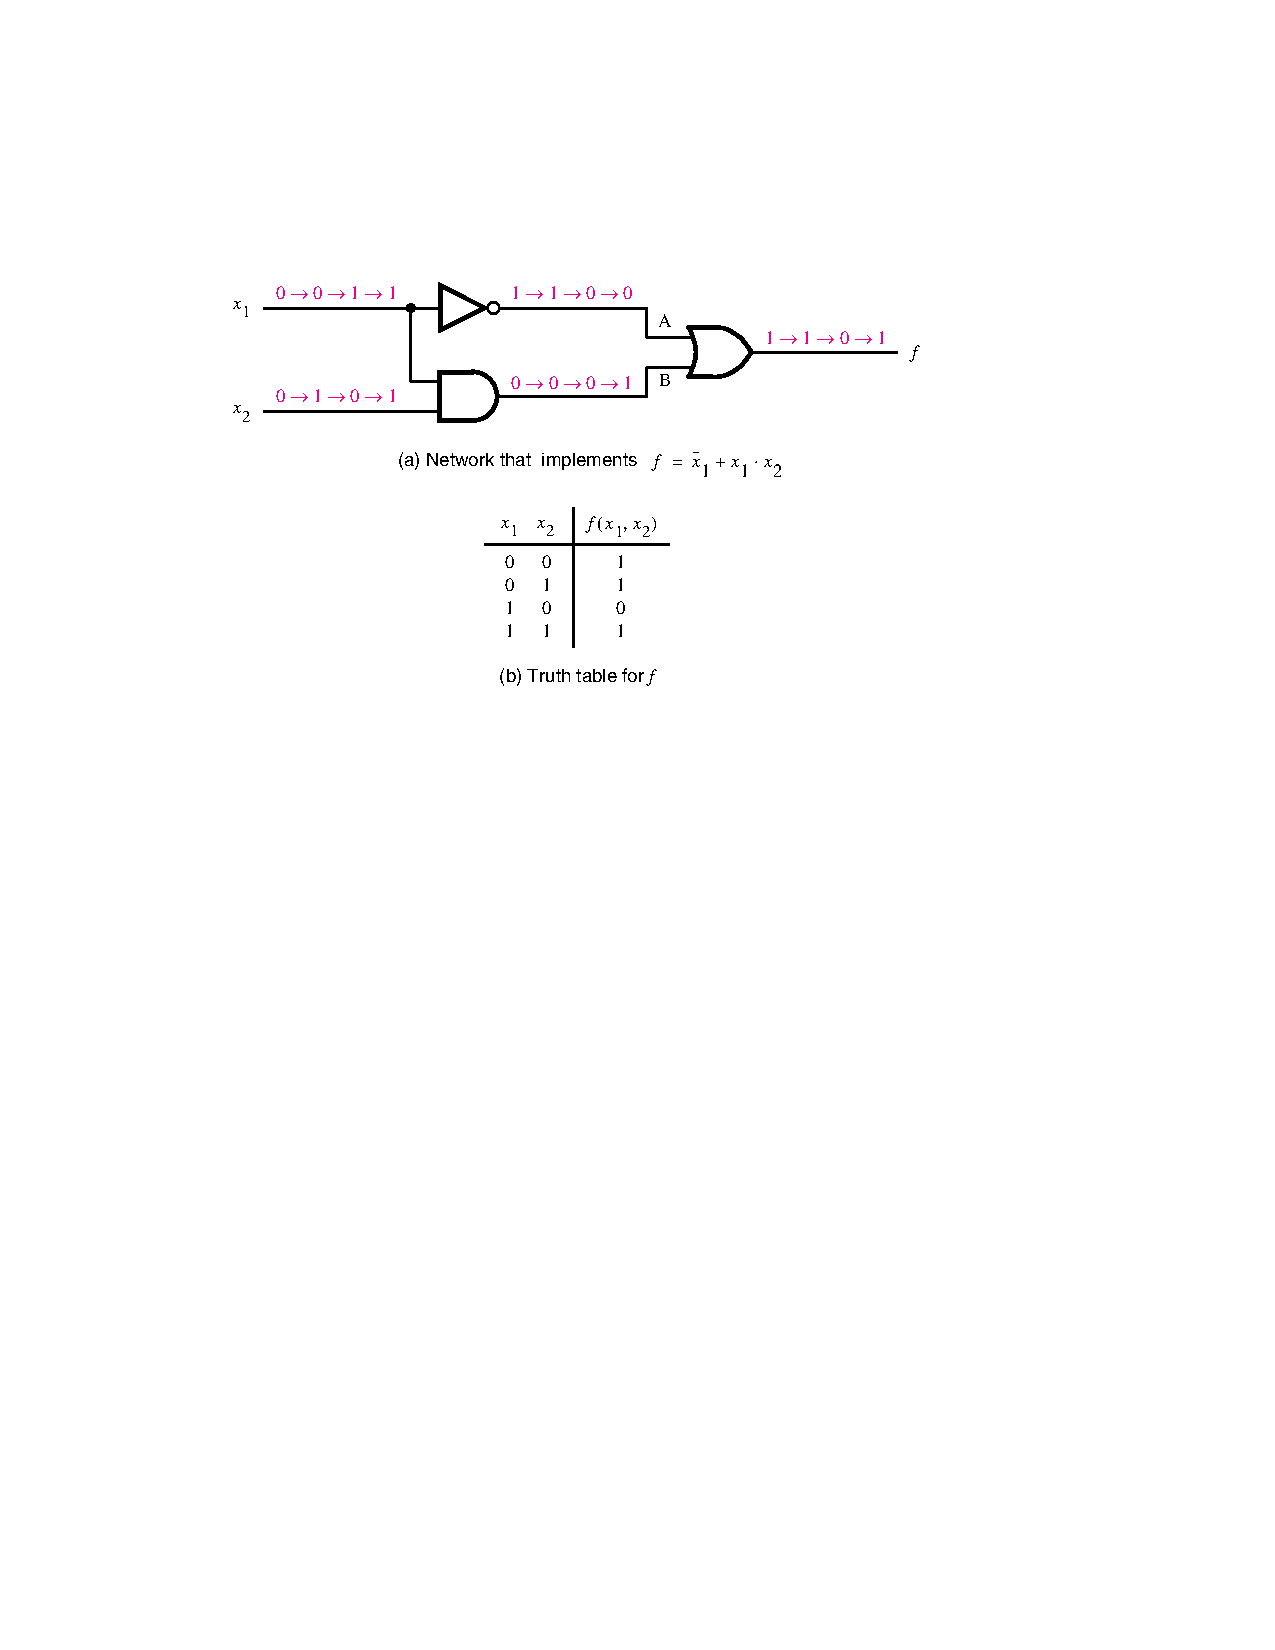
\includegraphics[width=.77\textwidth]{VerilogFig2_10ab}};
% \draw[step=0.25cm,gray,very thin] (0,0) grid (10.5,6.25);
% \draw[step=1cm,black,very thin] (0,0) grid (10.5,6.25);
\onslide<1>{
\draw[foo] (0.75,4.25) rectangle (1.25,4.75); % x2
\draw[foo] (0.75,5.75) rectangle (1.25,6.25); % x1
\draw[foo] (4.25,5.75) rectangle (4.75,6.25); % /x1
\draw[foo] (4.25,4.5)  rectangle (4.75,5); % x1.x2
\draw[foo] (8,5.2) rectangle (8.5,5.7); % f
\draw[foo] (5.75,1.8) rectangle (6.25,2.3); % t
\draw[foo] (8.25,5.2) to[bend left] (6.25,2.15); % seta \
}
\onslide<2>{
\draw[foo] (1.25,4.25) rectangle (1.75,4.75); % x2
\draw[foo] (1.25,5.75) rectangle (1.75,6.25); % x1
\draw[foo] (4.75,5.75) rectangle (5.25,6.25); % /x1
\draw[foo] (4.75,4.5)  rectangle (5.25,5); % x1.x2
\draw[foo] (8.5,5.2) rectangle (9,5.7); % f
\draw[foo] (5.75,1.5) rectangle (6.25,2); % t
\draw[foo] (8.75,5.2) to[bend left] (6.25,1.75); % seta \
}
\onslide<3>{
\draw[foo] (1.75,4.25) rectangle (2.25,4.75); % x2
\draw[foo] (1.75,5.75) rectangle (2.25,6.25); % x1
\draw[foo] (5.25,5.75) rectangle (5.75,6.25); % /x1
\draw[foo] (5.25,4.5)  rectangle (5.75,5); % x1.x2
\draw[foo] (9,5.2) rectangle (9.5,5.7); % f
\draw[foo] (5.75,1.25) rectangle (6.25,1.75); % t
\draw[foo] (9.25,5.2) to[bend left] (6.25,1.5); % seta \
}
\onslide<4>{
\draw[foo] (2.25,4.25) rectangle (2.75,4.75); % x2
\draw[foo] (2.25,5.75) rectangle (2.75,6.25); % x1
\draw[foo] (5.75,5.75) rectangle (6.25,6.25); % /x1
\draw[foo] (5.75,4.5)  rectangle (6.25,5); % x1.x2
\draw[foo] (9.5,5.2) rectangle (10,5.7); % f
\draw[foo] (5.75,0.8) rectangle (6.25,1.3); % t
\draw[foo] (9.75,5.2) to[bend left] (6.25,1); % seta \
}
\end{tikzpicture}%
}

\frame{     \centering
    \frametitle{Síntese de uma função lógica}
    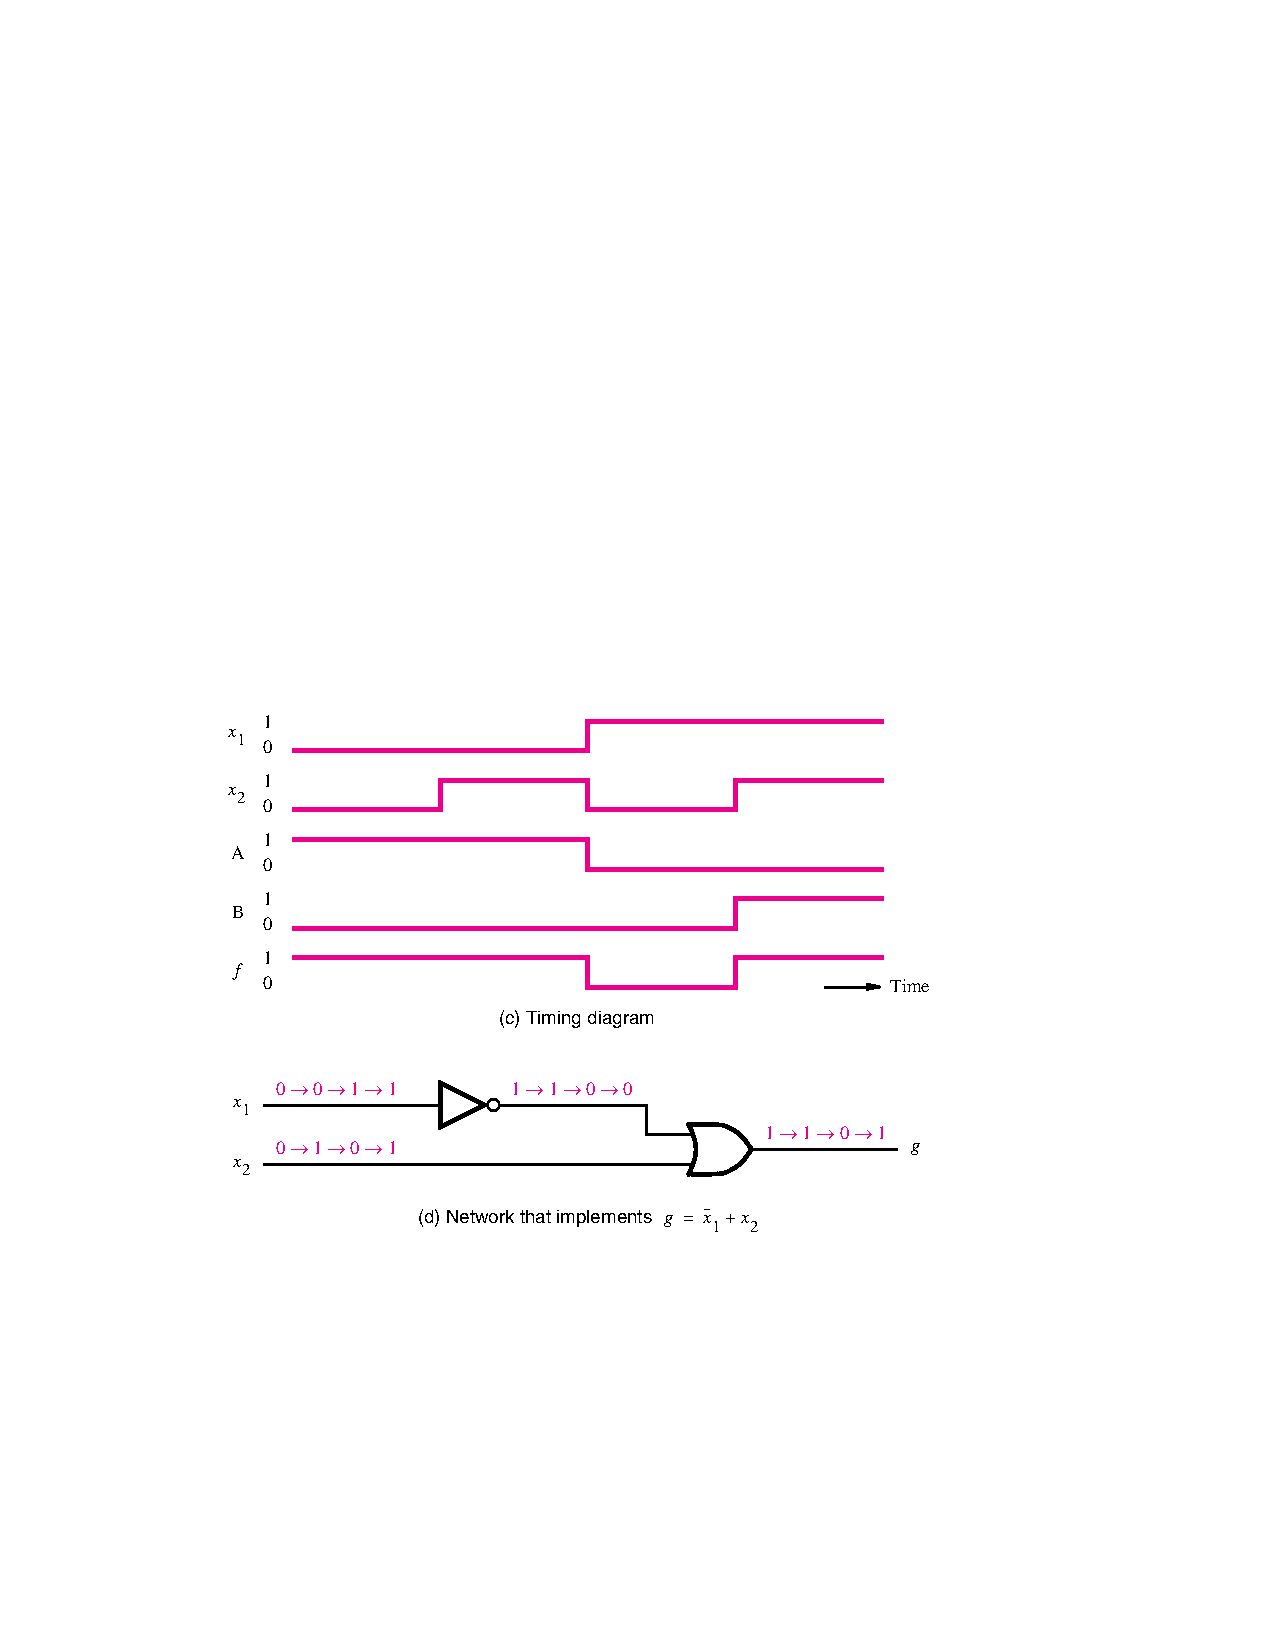
\includegraphics[scale=.7]{VerilogFig2_10cd}
}
%NOTE: se notarmos veremos que esta função é equivalente à anterior, e mais fácil de ser implementada. 

\frame{     \centering
    \frametitle{Funções lógicas equivalentes}
    \begin{itemize}
        \item Em geral, uma função lógica pode ser implementada com uma variedade de circuitos com diferentes custos; 
        \item As funções lógicas vistas anteriormente são funcionalmente equivalentes; 
        \item É possível notar a equivalência a partir da análise dos circuitos e contrução das tabelas verdade;
        \item 0 mesmo resultado pode ser alcançado através da manipulação algébrica de expressões lógicas, que fornece a base para técnicas modernas de projeto.
    \end{itemize}
}

\frame{     \centering
    \frametitle{Função XOR}
    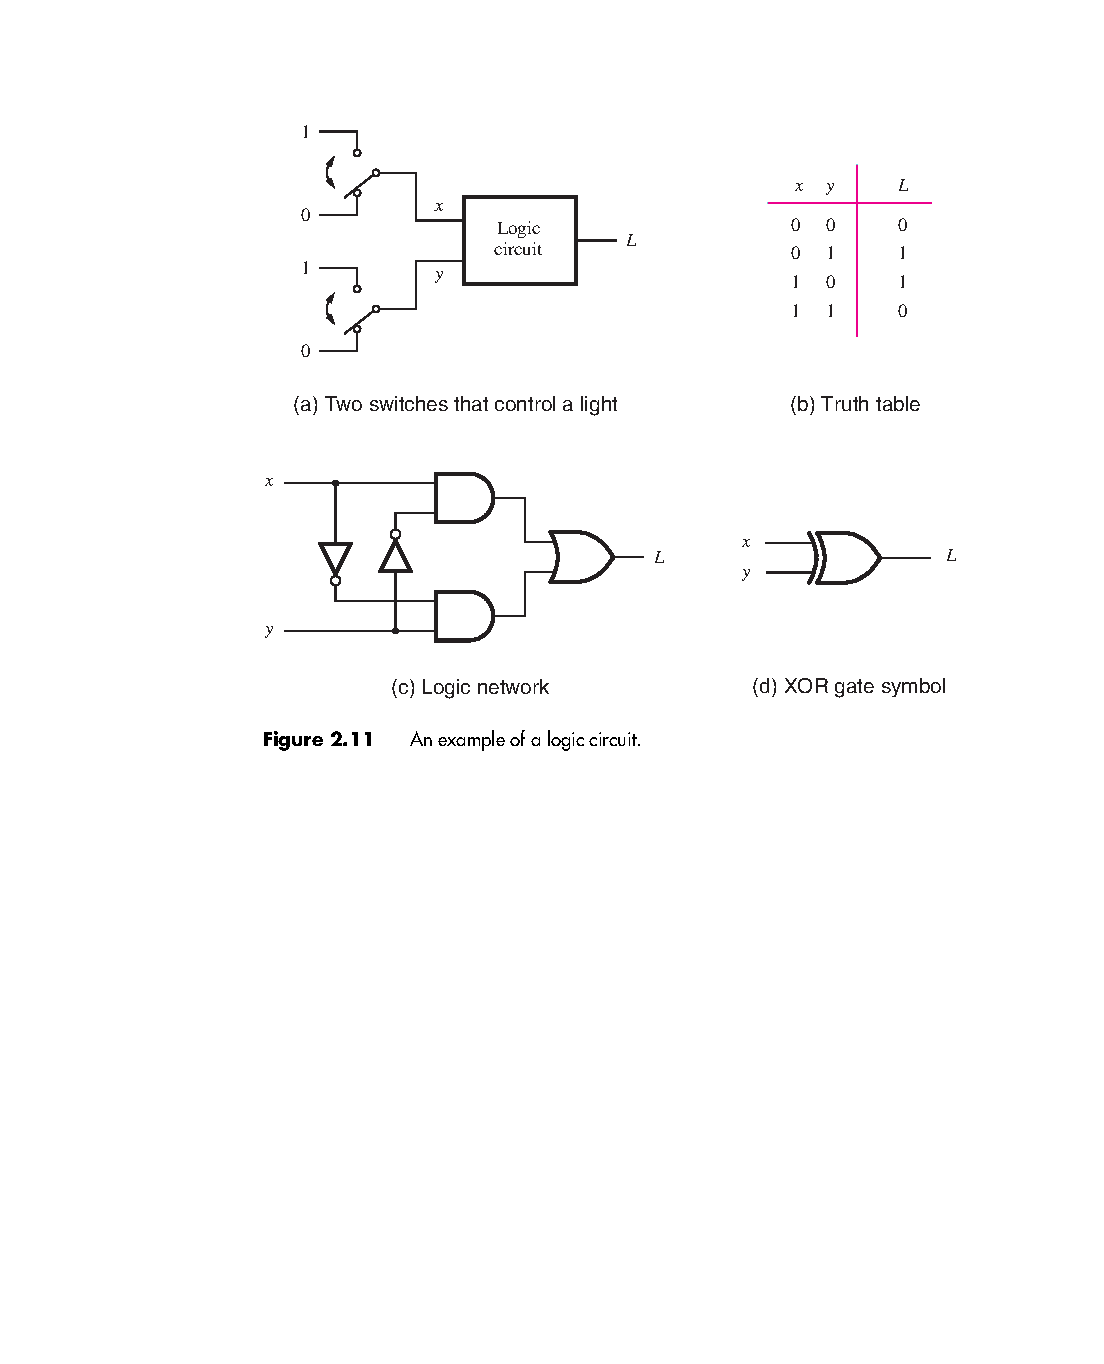
\includegraphics[scale=.7]{VerilogFig2_11} \\
    $L=f(x,y)=x \oplus y$
}

\frame{     \centering
    \frametitle{Aplicação: meio somador}
    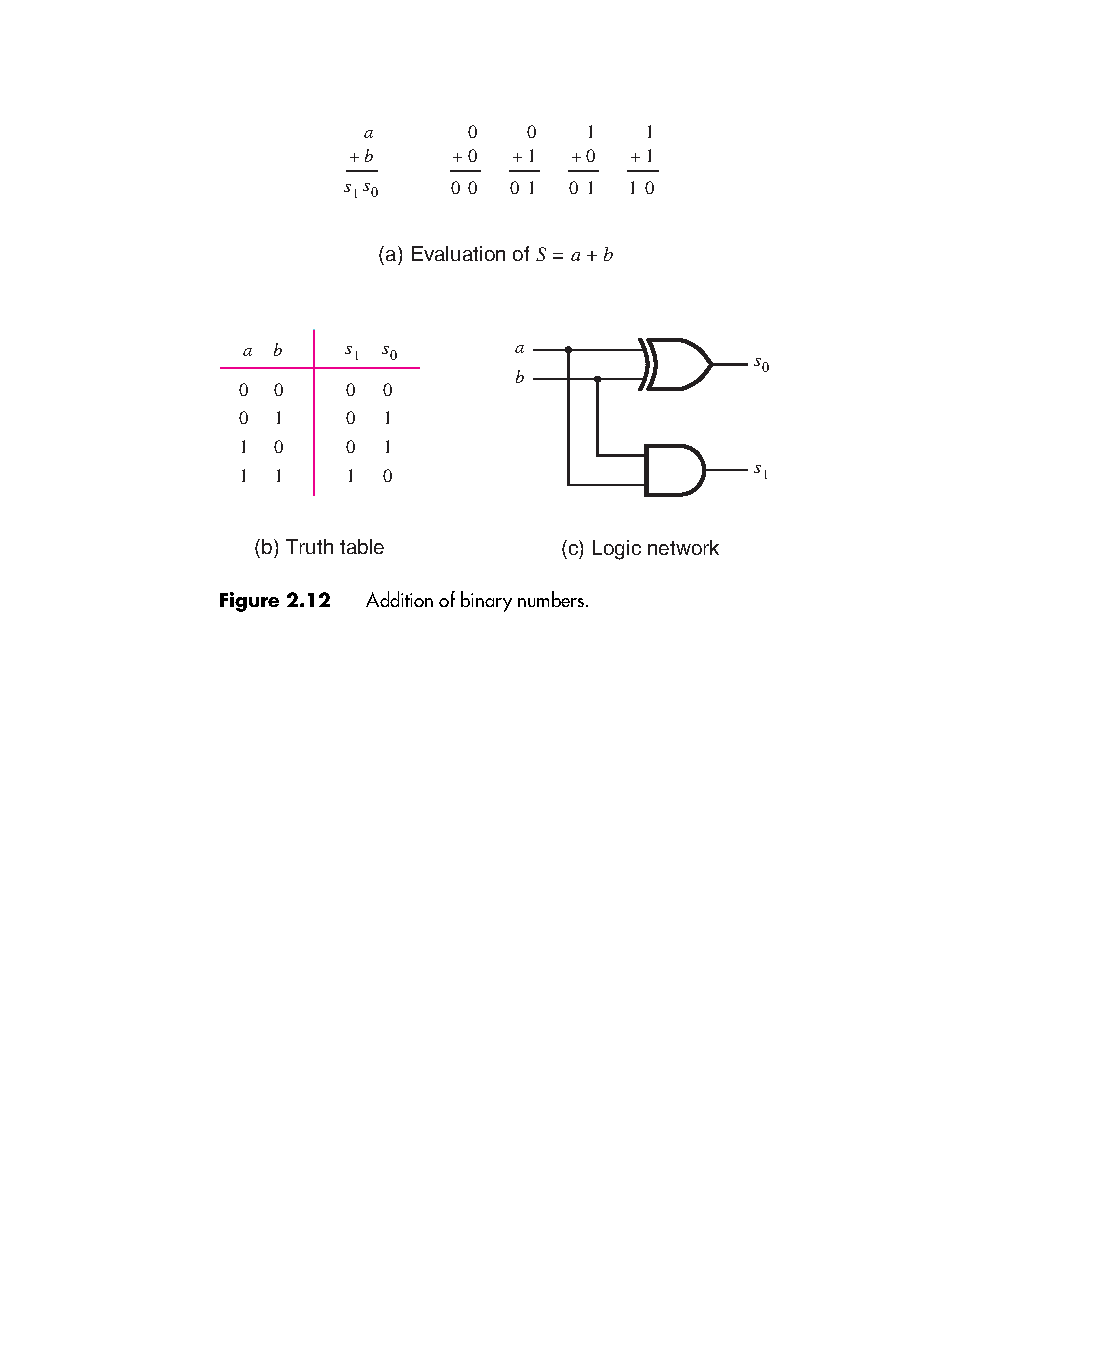
\includegraphics[scale=.7]{VerilogFig2_12} \\
    $S_0=f(a,b)=a \oplus b$ \\
    $S_1=f(a,b)=a.b$ 
}


\section{Bibliografia} %%%%%%%

\begin{frame}{\insertsection} 
	\begin{itemize}
		\item \href{https://www.google.com.br/search?q=filetype\%3Apdf+Fundamentals+of+Digital+Logic+with+Verilog+Design+&oq=filetype\%3Apdf}{Brown, S. \& Vranesic, Z. - Fundamentals of Digital Logic with Verilog Design, 3rd Ed., Mc Graw Hill, 2009}
		\item \href{http://ecalculo.if.usp.br/ferramentas/logica/logica.htm}{http://ecalculo.if.usp.br/ferramentas/logica/logica.htm}
	\end{itemize}
\end{frame}

\begin{frame}
	\titlepage
\end{frame} 

\end{document}